\chapter{Prospecting Algorithm}
\label{chapter:prospection}
Prospecting a swarm is one of the key elements of credit mining system. The prospecting module can be divided into two main stage, named \textit{probing} and \textit{mining} stage. Both of the stages rely on the swarm measurement by looking at its evolution \cite{2013:swarmevolution:su}. Credit mining system \textit{translates} the peer information it receives to predicted number of potential seeder and leecher. It also stores the \textit{availability} and rarest piece of the swarm by looking at the pieces possessed by each peers. 

When a swarm is marked as potential source of investment, credit mining system will extensively fetch information of that swarm in \textit{probing stage}. It only executed once and then decides whether the swarm is accepted or discarded. If the swarm is accepted and is possible to get the return of investment, credit mining system activate the \textit{mining stage}. This stage runs periodically as long as the system still running. The combination of both stages resulting the whole prospecting algorithm. 

\section{Probing stage}

Probing stage is important to decide which swarm that need to be mined. Wrong or sub-optimal decision will lead to low gained credit and less effect on the swarm. If a miner is given the wrong swarms, unnecessary overhead will likely to occur for just joining, putting investment, and extracting information from them. 

The challenge of probing is the limited and unverified information of the newly discovered swarm. Mindlessly download and participate in the swarm may waste the resource we have. Given a large number of swarms, it is impossible to mine all of them and get good results. A method to filter those swarms is essential in credit mining system. Some swarms might not complete (no one has complete files), only have \textit{webseeds}, or have invalid or duplicate content. Therefore, in credit mining system, we proposed the procedure called \textit{predownloading}. On top of that, to both tackle the tracker unavailability and get thorough swarm information, the mechanism to predict swarm health just by looking at the peers is necessary.

\begin{algorithm}[h!]
	\caption{\textit{Predownload} procedures}
	\label{alg:predown}
	\begin{algorithmic}[1]
		\Function{Predownload}{$infohash$, $n$}
		\If{$|download\_queue| > $ 100}	
		\State recall \Call{PREDOWNLOAD}{$infohash$, $n$}
		\EndIf
		\State \Call{push}{$download\_queue$, $infohash$}
		\State \Call{set\_pieces}{$infohash$, 0, 0}
		\State \Call{unset\_pieces}{$infohash$, $1$, \Call{pieces}{$infohash$}}
		\State \Return \Call{check\_predownload}{$infohash$, $n$}
		\EndFunction
		
		\Statex
		\Function{check\_predownload}{$infohash$, $n$}
		\State $peerlist \gets$ \Call{get\_peers}{$infohash$}
		\State \Call{add\_to\_peerlib}{$peerlist$}
		\If{wait long enough $and$ not finished yet}
		\State \Call{pop}{$download\_queue$, $infohash$}
		\State \Return False
		\EndIf
		
		\If{wait long enough $and$ already finished}
		\State \Call{translate\_peer}{\Call{get\_peerlib}{\null}}
		\State \Call{pop}{$download\_queue$, $infohash$}
		\State \Return True
		\EndIf
		\If{\Call{piece\_downloaded}{$infohash$} = $1$}
		\State $rarest\_pieces \gets$ \Call{find\_rare\_piece}{\Call{get\_peerlib}{\null}, $n$}
		\ForAll{$rarest\_pieces$ \textbf{as} $p$} 
			\State \Call{set\_pieces}{$infohash$, $p$, $p$}
		\EndFor
		\ElsIf{\Call{piece\_downloaded}{$infohash$} $\geq n$}
		\State mark $infohash$ as finished
		\EndIf
		\State \Return \Call{check\_predownload}{$infohash$, $n$}
		\EndFunction		
	\end{algorithmic}
\end{algorithm}

\textit{Predownloading} is a means to download a predefined number of pieces in a particular torrent in such a way that it only consumes small portion of resource while trying to get as much information as possible of the swarm. Pseudocode of this procedures shown in Algorithm \ref{alg:predown}. Assume that there are $n$ pieces that need to be \textit{predownloaded}. To be able to join swarms, the pieces that intended to be downloaded need to be stated. Although any piece will do, we choose only the first piece. Picking the first piece can result a smaller storage allocation. The system will then look for $n - 1$ rarest pieces available in the swarm and reject the rest of the pieces. By finding rarest pieces, it can filter more swarm. Moreover, this method is consistent with the \bt~core functions. While \textit{predownloading}, the system actively ask for new peers to tracker or DHT and store it afterwards. The mining activity will continue at the point where \textit{predownloading} finished. 

\subsection{Finding rare pieces}
The existence of rarest pieces is one of the important aspect for both \bt~and credit mining system. Rarest piece is a piece that has minimum number of peer who owned it. Note that rarest pieces is not necessarily only one in the whole swarm. Piece usually identified by its index. Algorithm \ref{alg:rarepc} shows how to find those pieces. This algorithm receives known peer list and the number of desired piece as parameter. It will return the list of rarest pieces in the swarm. 

\begin{algorithm}[h]
	\caption{Finding rare pieces procedures}
	\label{alg:rarepc}
	\begin{algorithmic}[1]
		\Require{$plist$ as list of stored peers}
		\Require{$n$ as desired rare pieces amount}
		
		\Function{find\_rare\_piece}{$plist, n$}
		\State $mbit \gets \Call{populate\_piece}{plist}$
		
		\If{$\Call{min}{mbit} = \Call{max}{mbit}$}
			\State \Return [] \label{alg:rarepc:err1}
		\EndIf
		\State $rbit \gets mbit$ where its value equal to $\Call{min}{mbit}$ \label{alg:rarepc:err2}
		\State remove owned piece from $rbit$ \label{alg:rarepc:err3}
		\State $ret \gets$ choose randomly maximum $n$ piece from $rbit$ \label{alg:rarepc:err4}
		\State \Return $ret$
		\EndFunction
		\Statex
		\makeatletter\setcounter{ALG@line}{0}\makeatother
		\Function{populate\_piece}{$plist$}
		\State $ret \gets []$
		\ForAll{$p$ in $plist$}
		\ForAll{$pc$ in \Call{get\_pieces}{$p$}}
		\State $ret[pc]$++
		\EndFor
		\EndFor
		\State \Return $ret$
		\EndFunction
	\end{algorithmic}
\end{algorithm}

In Algorithm \ref{alg:rarepc}, there are several cases in which rarest pieces could not be found. Variable $mbit$ contains the number of peer that has a particular piece. Minimum value of $mbit$ means the number of peers that has rarest piece. In line \ref{alg:rarepc:err1}, it means that all the pieces has been owned by all peers. In line \ref{alg:rarepc:err2}, there is  possibility that $mbit$ is empty. For example if there is no information of peers or pieces. Line \ref{alg:rarepc:err3} also can strip $rbit$ to empty if by any chance the system already had all the rarest pieces. Lastly, in line \ref{alg:rarepc:err4} it is possible that the number of rarest piece is less than $n$. In this case, the difference between $n$ and $|ret|$ will be computed in the next turn. 

\subsection{Peer translation}
For able to be fully decentralized, it is important to not rely on the tracker. Instead, trackless \bt~environment described in 2008 which contains DHT protocol \cite{2008:dht:loewenstern} and magnet link\cite{2008:magnet:hazel} are recommended. In case of multi-tracker\footnote{Defined in : \url{http://www.bittorrent.org/beps/bep_0012.html}.}, some swarms may have entirely different number of seeder and peers for each of the tracker like shown in figure \ref{fig:diffsr}. Because of this reason, we alternate the swarm information source by looking directly from the connected peers. We called the procedure to interpret swarm information from both currently and previously connected peers as \textit{peer translation}. 

\begin{figure}[ht]
	\centering
	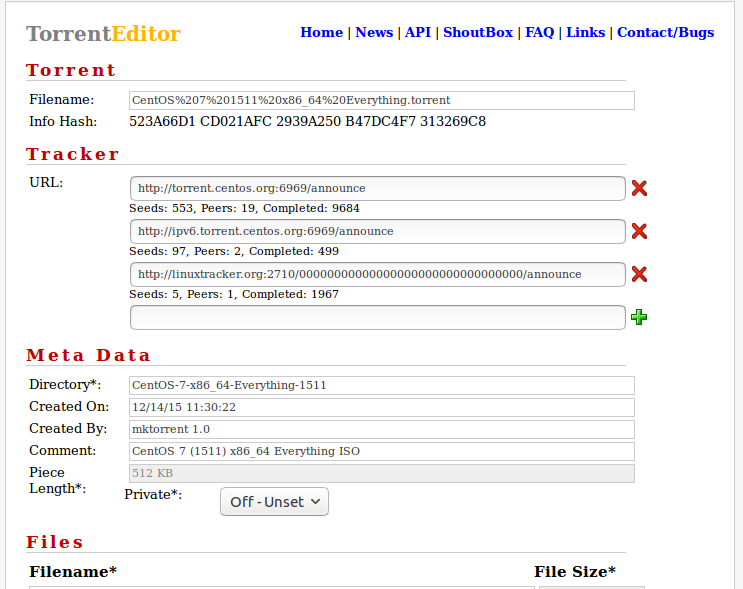
\includegraphics[width=0.7\textwidth]{pics/diffsr.png}
	\caption{Different number of seeder and peers/leecher reported by different trackers.}
	\label{fig:diffsr}
\end{figure}

The \textit{peer translation} receives list of peers as input and returns the predicted number of seeder and downloader. This procedure is shown in Algorithm \ref{alg:peertrans1}. We categorize a peer is a seeder if it satisfy at least one of three conditions. The conditions are: it only wants to upload right now, it is 80\% finished with its download, and it is known to upload more data to us than download. Whichever category gives the highest number will be picked. 

In the other hand, we define a peer is a leecher if it satisfies at least one of three conditions : it is currently interested in our pieces, its download process still under 80\% and not declaring as ``upload only'', and it is known to download more data from us than uploading. Likewise, any category gives the highest number will be picked. Finally, both projected number of seeder an leecher will be returned to the caller.

\begin{algorithm}[t]
	\caption{Peer translation algorithm}
	\label{alg:peertrans1}
	\begin{adjustwidth}{}{-0.3cm}
	\begin{algorithmic}[1]
	\Function{translate\_peer}{$peer\_list$}
		\State{$num\_seeder \gets 0$}
		\State{$num\_leecher \gets 0$}
		\Statex
		\State{$upload\_only \gets |$\Call{get\_peer}{$UPLOAD\_ONLY$}$|$}
		\State{$finished \gets |$\Call{get\_peer}{$PROGRESS >$ 0.8}$|$}
		\State{$unfinish \gets |$\Call{get\_peer}{$\neg UPLOAD\_ONLY$ \& $PROGRESS < $0.8}$|$}
		\State{$interested \gets |$\Call{get\_peer}{$INTERESTED$}$|$}
		\State $num\_seeder \gets $ \Call{max}{$upload\_only$, $finished$}
		\If{$num\_seeder = 0$}	
		\State $num\_seeder \gets $ number of peer which downloaded $>$ uploaded
		\EndIf
		\State $num\_leecher \gets $ \Call{max}{$interested$, $unfinish$} \label{alg:peertrans1:pickleech}
		\If{$num\_leecher = 0$}	
		\State $num\_leecher \gets $ number of peer which uploaded $>$ downloaded
		\EndIf
		\State \Return $num\_seeder$, $num\_leecher$
		\EndFunction
	\end{algorithmic}
	\end{adjustwidth}
\end{algorithm}

\section{Mining stage}
After the probing has been done, the mining stage will take place regularly. Mining stage occurred when the credit mining system already decide which swarm that need to be mined. In a fixed interval, the system evaluates the swarms in \textit{swarm selection} algorithm. It is based on \textit{selection policy} which determines the criteria that need to be considered. We explored the currently implemented policy in \ref{section:swarmselect}. All the miner need to comply to one defined policy. In all policies, swarm with low prospect will be paused, and one with higher prospect replace the old one. Paused swarm may be chosen again in the future. Likewise, the miners may always stick with swarms with very good prospect. As a contribution, we proposed \textit{scoring policy} that will be elaborated more in \ref{section:scorepolicy}.

Credit mining system monitors those swarm continuously. The purpose is to look for swarms that are not well-performed in a particular time frame. Under certain requirements, this swarm then will be \textit{stimulated} by optimistically download few rare pieces at one time. Objective of this approach is to eliminate idleness caused by bottleneck of share mode. This approach will be elaborated in \ref{section:swarmstimulate}.

\subsection{Swarm Selection}
\label{section:swarmselect}
The number of swarm for a single source should not be limited. However, with limited resource one may want to limit the number of active swarms at a time. Swarm selection is the process of selecting swarm based on its mining potential. The selection need to be run periodically because swarm information is constantly changing. At some point, previously selected swarm may not beneficial to mine for both the miners and the community. Eventually, it has to be substituted by another swarm. Swarm selection process is controlled by the applied policy. The policy contains rules to sort which swarm to start and stop.

Although it is possible for user to create their own policy, three policies have been defined on the preliminary work \cite{2015:creditmining:capota}. Those are based on random, swarm age, and seeder ratio. \textit{Random policy} mostly used as the baseline of the experiment. \textit{Swarm Age policy} is claimed better than random policy. It selects the swarm based on its age. New published swarm known to have higher demand than other type of swarm \cite{2012:economicbt:kash}. With a lot of peer in early swarm, it will increase the chance to get more credit. \textit{Seeder Ratio policy} selects the swarm that has lower number of seeder relative to all the peers participated in this swarm. This policy is specialized to help undersupplied swarm. 

\subsection{Scoring Policy}
\label{section:scorepolicy}
In this thesis, we intend to extend those policies so it can be highly customizable and balance credit gaining and helping undersupplied swarm. We propose a policy named \textit{scoring policy} to tackle this issue. Scoring policy was brought up with seeder ratio policy as its base. It offers a method to quantify swarm prospect and to reduce possible identical result from two swarms or more. It can be customized with its \textit{score multiplier}. The idea behind this policy is to give higher score for swarm which has lower seeder ratio, has more peers, lower piece availability, and many activities detected in the swarm. Higher score means getting higher priority to be mined.

Scoring policy consists of several features. First is the seeder ratio. As mentioned before, it is useful to measure whether a swarm is undersupplied or not. This is particularly useful to \textit{help} a swarm. Lower seeder ratio should get higher priority in mining. Second is the number of peer in a swarm. In small swarm, seeder ratio may not relevant because there is not any significant difference between one and another. In a case where ratio of seeder and peers is almost equal for all swarms, it is useful to target large swarms instead of the small one as there are comparably more options to give our pieces to. Third aspect is the file availability of the swarm. In flashcrowd case swarm, there are a significant amount of peers who do not have a large portion of the file. Comparing this to another swarm which most of the leecher almost finished their download, mining flashcrowd swarm will give higher credit and more beneficial to the community altogether. Last element that we considered is the activity of a swarm. It is preferable to mine a swarm whose some of the peers already download or upload any data from or to us. Moreover, one which had faster speed is considered. The worst case happened when there is not any peer interested with the piece we already have. In the other hand, if a peer already interacted with us before, there is a chance we will get chosen again in the future. This feature incentivize swarm which had interacted with the miners previously.

\begin{algorithm}[th]
	\caption{Scoring policy algorithm}
	\label{alg:scorep}
	\begin{algorithmic}[1]
		\Require{$M\_leech$ as leecher multiplier}
		\Require{$M\_pratio$ as peer ratio multiplier}
		\Require{$M\_avail$ as peer availability multiplier}
		\Require{$S\_low$ as extra score for lower activity}
		\Require{$S\_high$ as extra score for higher activity}
		\Statex
		\Require{$peerlist$ as the list of stored peers}
		\Require{$swarmlist$ as the list of swarm in the miners}
		\Statex
		\ForAll{$s \in swarmlist$}
			\State{$rleech \gets 1 - $\Call{seeder\_ratio}{s}}
			\State{$rpeer \gets |$\Call{peers}{s}$|/|peerlist|$}
			\State{$ravail \gets 1 - $\Call{availability}{s}$/|peerlist|$}
			\State{$score[s] \gets M\_leech*rleech + M\_pratio * rpeer + M\_avail * ravail$}			\State $total\_speed[s] \gets 0$
			\ForAll{$p \in $\Call{peers}{$s$}}
				\State $total\_speed[s] \gets total\_speed[s] + \Call{get\_speed}{p}$
			\EndFor
		\EndFor
		\State \Call{sort}{$total\_speed$}
		\ForAll{$s \in swarmlist$}
			\If{$index(total\_speed, s) < |total\_speed|/2$}
				\State $score[s] \gets score[s] + S\_low$
			\Else{\null}
				\State $score[s] \gets score[s] + S\_high$
			\EndIf
		\EndFor
		\State \Return{$score$}
	\end{algorithmic}
\end{algorithm}

Scoring policy, as shown in Algorithm \ref{alg:scorep}, starts with examining all the swarm registered in a miner. Then it decides the score individually as shown in line 2-5. Variable $rpeer$ is the ratio of a number of peer in this swarm and total number of peers that already known from all the swarm. \textit{Availability} is the number of complete copies of a piece plus the fraction of non-seeder peer that provide a subset of a piece. Its algorithm is explored in Algorithm \ref{alg:savail}. For \textit{availability} to be 0 it means that there is not any single piece from any of the discovered peers. It will also return 0 in a case where the piece/peer information could not be received. If all the peer has completed files, \textit{availability} will reach its maximum value which is equal to the number of discovered peer. After the individual score was assigned, the activity of each peer on each of the swarm is calculated. The activity, which identified by total download speed a remote peer to the miner, is sorted increasingly by its speed. Then, first half of the sorted activity is marked as low activity, and given the lower activity score (line 14). Similarly happens with second half of the list, but with higher activity and higher score (line 16).

\begin{algorithm}[h]
	\caption{Swarm availability}
	\label{alg:savail}
	\begin{algorithmic}[1]
		\Require{$plist$ as list of stored peers}
		\State $mbit \gets \Call{populate\_piece}{plist}$
		\State $complete\_peer \gets |\Call{get\_seeder}{\null}|$ 
		\State $min\_peer \gets \Call{min}{mbit}$
		\State $more\_piece \gets $ number of piece which has more peer than $min\_peer$
		\State \Return $complete\_peer + min\_peer + more\_peer/|mbit|$
	\end{algorithmic}
\end{algorithm}

Scoring policy is designed in such a way so that it can be easily customized based on user preferences. This can be done by providing value to the multiplier and activity incentive: $M\_leech$, $M\_pratio$, $M\_avail$, $S\_low$, and $S\_high$. Changing the multiplier will affect its behavior. For example, if a user do not consider number of peers is important, he can set the multiplier for $M\_pratio$ as 0. Setting other parameter except $M\_leech$ as 0 will make scoring policy behave like seeder ratio policy. Similarly, setting other parameter except $M\_avail$ as 0 will prioritize swarm with very low availability. This behavior is similar as if it is applied with swarm age policy in flashcrowd case.

\subsection{Swarm stimulation}
\label{section:swarmstimulate}
As mentioned in Section \ref{section:sharemode}, activating \textit{share mode} can result in a bottleneck, especially in the beginning of joining a swarm. \textit{Predownload} a swarm, if handled correctly, can solve this issue in probing stage. By downloading several rarest pieces beforehand, the chance those are going to be uploaded is high. Therefore, positive upload/download ratio is likely, thus, avoiding the \textit{share mode} bottleneck. However, there is not any guarantee when the system is on mining stage.

We introduced a method to stimulate the mining activity on idle swarms. It starts by looking which swarm that already idle for some amount of time. Those swarm are now suspected for in the \textit{stale} state. We then download several rarest pieces on that swarm. We called these pieces \textit{stimulant}. The stimulant can be downloaded only if the share ratio for this swarm is higher than the predefined threshold. This threshold should be lower than \texttt{share\_mode\_target} as in both credit mining system and \textit{libtorrent}. If the ratio is already too low, miners should wait for a piece to be uploaded first. Then, if it is not possible, then this swarm will be blacklisted in the next round and be substituted by another swarm. This process is called \textit{stimulating} the swarm. By optimistically download rarest piece simultaneously, we hope to stimulate the mining activity in the long term.